\chapter{Proposta}
\label{ch:proposta}

\lipsum[5] Conforme Figura \ref{fig:exemplo-1}.

\begin{figure}[h!]
  \centering
  \Caption{\label{fig:exemplo-1} Lorem ipsum dolor sit amet.}	
  \UECEfig{}{
  \fbox{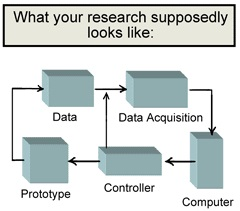
\includegraphics[width=8cm]{figuras/figura-1}}
		}{
  \Fonte{Elaborado pelo autor}
		}	
\end{figure}

\lipsum[5] Conforme Código-fonte \ref{lst-codigoCsharp}.

\begin{lstlisting}[language={[Sharp]C}, label={lst-codigoCsharp}, caption={Enumeração}]
public enum ETipoComando
{
  TIPO_0 = 0, 
  TIPO_1 = 1, // tipo 1 
  TIPO_2 = 2, // declaração do tipo 2
}
\end{lstlisting}

% \lipsum[2] Conforme Algoritmo \ref{alg:algoritmo}. 

% \begin{algorithm}[!ht]
%   \Caption{Exemplo de Algoritmo \label{alg:algoritmo}}
%   \SetSpacedAlgorithm
%   \ForAll{algoritmo  $Al$}{
%     Criar primeira ação do algoritmo $Al$\;
%     Criar segunda ação\;
%     \textbf{call} $executarComando$($Alg$)\;
%     Fazer ação 1\;
%     Fazer ação 2\;
%     Fazer ação 3\;
%     \If{possuiCondicao($Alg$)} {
%       Fazer ação 4\;
%     }
%   }  
%   \DontPrintSemicolon
%   \SetKwFunction{FMain}{$executarComando$}
%   \SetKwProg{Fn}{Function}{:}{}
%   \Fn{\FMain{$Alg$}}{
%     \ForAll{comando $Cp$ de $Alg$ }{
%       Executar comando $Cp$\;  
%     }
%   }

% \end{algorithm}

\lipsum[2] Conforme Algoritmo \ref{alg:exemplo-de-algoritmo}. 


\begin{algorithm}[!ht]
  \SetAlgoLined
  \Caption{\label{alg:exemplo-de-algoritmo}Como escrever algoritmos no \LaTeX2e}
  \SetSpacedAlgorithm
  \Entrada{o proprio texto}
  \Saida{como escrever algoritmos com \LaTeX2e }
  \Inicio{
    inicializa\c{c}\~ao\;
    \Repita{fim do texto}{
      leia o atual\;
      \Se{entendeu}{
        vá para o próximo\;
        próximo se torna o atual\;
        \textbf{chamar} $funcaoCom$($Parametro$)\;
      }
      \Senao{volte ao início da seção\;}
      }
  }

  \DontPrintSemicolon
  \SetKwFunction{FuncaoAuxiliar}{$funcaoCom$}
  \Funcao{\FuncaoAuxiliar{$Parametro$}}{
      \ParaTodo{elemento $p$ do $Parametro$}{
        imprimir $p$\;  
      }
    }
\end{algorithm}